\documentclass{article}
\usepackage[utf8x]{inputenc}
\usepackage[T1, T2A]{fontenc}
\usepackage[russian]{babel}
\usepackage{amsmath}
\usepackage{amssymb}
\usepackage{graphicx}
\setlength\parindent{0pt}
\usepackage[parfill]{parskip}
\pagenumbering{gobble}

\begin{document}
На картинке ниже изображены градиенты бесконечно гладкой функции $f(x,y)$ в узлах решетки с шагом $0.5$ (вектор исходит из той точки, в которой вычисляется градиент).
\begin{figure}[h]
\center{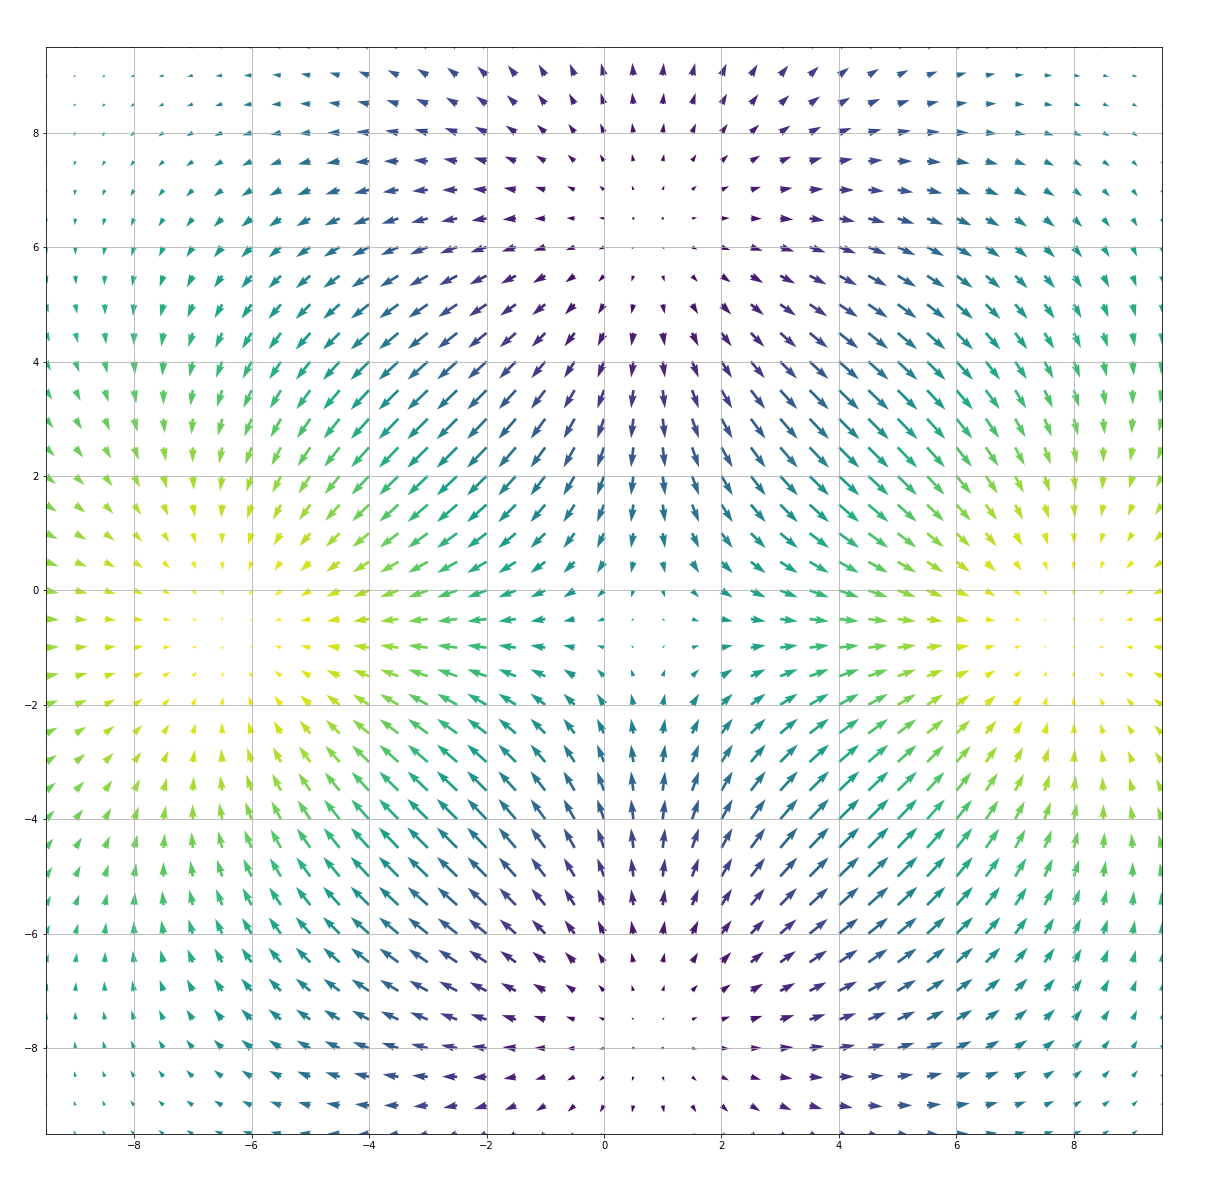
\includegraphics[width=\textwidth]{gradients}}
\end{figure}

Утверждается, что существуют прямые (более одной), вдоль которых матрица вторых производных
$$\left( \begin{array}{cc} \frac{\partial^2 f}{\partial x^2}& \frac{\partial^2 f}{\partial x \partial y}\\ \frac{\partial^2 f}{\partial x \partial y}&\frac{\partial^2 f}{\partial y^2} \end{array} \right)$$
вырождена.\\
(a) Найдите и укажите их количество и угловые коэффициенты (то есть коэффициенты $a$ в уравнении $y = ax + b$).\\
(b) Верно ли, что существуют точки, в которых градиент не равен нулю, но, стартовав из которых, нельзя с помощью градиентного спуска прийти в точку минимума?
\end{document}
